\title{Unsupervised learning}

\subsection{Unsupervised learning}

In unsupervised learning, the task is to infer hidden structure from
unlabeled data, comprised of training examples $\{x_n\}$.

We demonstrate how to do this in Edward with an example.
The script is available
\href{https://github.com/blei-lab/edward/blob/master/examples/tf_mixture_gaussian.py}
{here}.


\subsubsection{Data}

Use a simulated dataset of 2-dimensional datapoints
$\mathbf{x}_n\in\mathbb{R}^2$.
\begin{lstlisting}[language=Python]
def build_toy_dataset(N):
  pi = np.array([0.4, 0.6])
  mus = [[1, 1], [-1, -1]]
  stds = [[0.1, 0.1], [0.1, 0.1]]
  x = np.zeros((N, 2), dtype=np.float32)
  for n in range(N):
    k = np.argmax(np.random.multinomial(1, pi))
    x[n, :] = np.random.multivariate_normal(mus[k], np.diag(stds[k]))

  return x

x_train = build_toy_dataset(500)
data = {'x': x_train}
\end{lstlisting}

We visualize the generated data points.
\begin{lstlisting}[language=Python]
plt.scatter(x_train[:, 0], x_train[:, 1])
plt.axis([-3, 3, -3, 3])
plt.show()
\end{lstlisting}
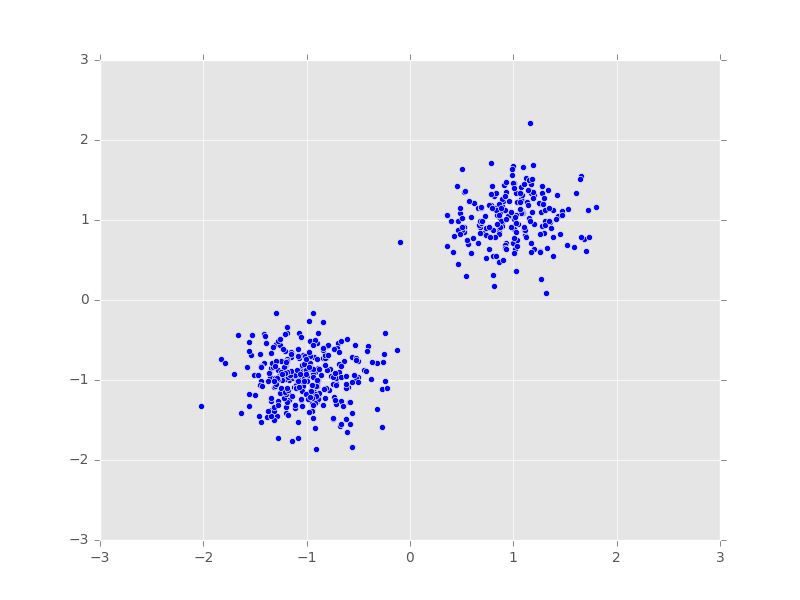
\includegraphics[width=700px]{/images/unsupervised-fig0.png}

\subsubsection{Model}

Posit the model as a mixture of Gaussians. For more details on the
model, see the
\href{/tutorials/mixture-gaussian}
{Mixture of Gaussians tutorial}.

Here we build the model in Edward using TensorFlow, and set the number
of mixture components to be 2.
\begin{lstlisting}[language=Python]
class MixtureGaussian:
  """
  Mixture of Gaussians

  p(x, z) = [ prod_{n=1}^N sum_{k=1}^K pi_k N(x_n; mu_k, sigma_k) ]
            [ prod_{k=1}^K N(mu_k; 0, cI) Inv-Gamma(sigma_k; a, b) ]
            Dirichlet(pi; alpha)

  where z = {pi, mu, sigma} and for known hyperparameters a, b, c, alpha.

  Parameters
  ----------
  K : int
    Number of mixture components.
  D : float, optional
    Dimension of the Gaussians.
  """
  def __init__(self, K, D):
    self.K = K
    self.D = D
    self.n_vars = (2 * D + 1) * K

    self.a = 1.0
    self.b = 1.0
    self.c = 3.0
    self.alpha = tf.ones([K])

  def log_prob(self, xs, zs):
    """Return scalar, the log joint density log p(xs, zs)."""
    x = xs['x']
    pi, mus, sigmas = zs['pi'], zs['mu'], zs['sigma']
    log_prior = dirichlet.logpdf(pi, self.alpha)
    log_prior += tf.reduce_sum(norm.logpdf(mus, 0.0, self.c))
    log_prior += tf.reduce_sum(invgamma.logpdf(sigmas, self.a, self.b))

    # log-likelihood is
    # sum_{n=1}^N log sum_{k=1}^K exp( log pi_k + log N(x_n; mu_k, sigma_k) )
    # Create a K x N matrix, whose entry (k, n) is
    # log pi_k + log N(x_n; mu_k, sigma_k).
    N = get_dims(x)[0]
    matrix = []
    for k in range(self.K):
      matrix += [tf.ones(N) * tf.log(pi[k]) +
                 multivariate_normal_diag.logpdf(x,
                 mus[(k * self.D):((k + 1) * self.D)],
                 sigmas[(k * self.D):((k + 1) * self.D)])]

    matrix = tf.pack(matrix)
    # log_sum_exp() along the rows is a vector, whose nth
    # element is the log-likelihood of data point x_n.
    vector = log_sum_exp(matrix, 0)
    # Sum over data points to get the full log-likelihood.
    log_lik = tf.reduce_sum(vector)

    return log_prior + log_lik


model = MixtureGaussian(K=2, D=2)
\end{lstlisting}


\subsubsection{Inference}
Perform variational inference.
%
The latent variables are the mixture probabilities,
component means, and component variances.
Define the variational model to be a Dirichlet $\times$ fully factorized normal
$\times$ fully factorized inverse Gamma.
%The latent variables are $\mathbf{z} = (\pi, \mu, \sigma)$.
%\begin{align*}
%  q(\mathbf{z} \;;\; \lambda)
%  &=
%  \text{Dirichlet}(\mathbf{z}_\pi)
%  \times
%  \text{Normal}(\mathbf{z}_\mu)
%  \times
%  \text{InverseGamma}(\mathbf{z}_\sigma)
%\end{align*}
%
%The model in Edward is
\begin{lstlisting}[language=Python]
qpi_alpha = tf.nn.softplus(tf.Variable(tf.random_normal([K])))
qmu_mu = tf.Variable(tf.random_normal([K * D]))
qmu_sigma = tf.nn.softplus(tf.Variable(tf.random_normal([K * D])))
qsigma_alpha = tf.nn.softplus(tf.Variable(tf.random_normal([K * D])))
qsigma_beta = tf.nn.softplus(tf.Variable(tf.random_normal([K * D])))

qpi = Dirichlet(alpha=qpi_alpha)
qmu = Normal(mu=qmu_mu, sigma=qmu_sigma)
qsigma = InverseGamma(alpha=qsigma_alpha, beta=qsigma_beta)
\end{lstlisting}

Run variational inference for 2500 iterations, using a batch
of 20 datapoints and 10 latent variable samples per iteration.
\begin{lstlisting}[language=Python]
inference = ed.KLqp({'pi': qpi, 'mu': qmu, 'sigma': qsigma}, data, model)
inference.run(n_iter=2500, n_samples=10, n_minibatch=20)
\end{lstlisting}
In this case
\texttt{KLqp} defaults to minimizing the
$\text{KL}(q\|p)$ divergence measure using the score function
gradient.
For more details on inference, see the \href{/tutorials/klqp}{$\text{KL}(q\|p)$ tutorial}.


\subsubsection{Criticism}

We visualize the predicted memberships of each data point.
We pick the cluster assignment which produces
the highest log-likelihood for each data point.
First we output a K x N matrix of log-likelihoods, per
per-cluster assignment $k$ and per data-point $\mathbf{x}_n$.

We do this by adding the \texttt{predict()} method in the
probability model.
\begin{lstlisting}[language=Python]
class MixtureGaussian:
  ...
  def predict(self, xs, zs):
    """Calculate a K x N matrix of log-likelihoods, per-cluster and
    per-data point."""
    x = xs['x']
    pi, mus, sigmas = zs['pi'], zs['mu'], zs['sigma']

    matrix = []
    for k in range(self.K):
      matrix += [multivariate_normal_diag.logpdf(x,
                 mus[(k * self.D):((k + 1) * self.D)],
                 sigmas[(k * self.D):((k + 1) * self.D)])]

    return tf.pack(matrix)
\end{lstlisting}
Then we evaluate the log-likelihood on the training data
and take the $\arg\max$ along the rows.
\begin{lstlisting}[language=Python]
log_liks = []
for s in range(100):
  zrep = {'pi': qpi.sample(()),
          'mu': qmu.sample(()),
          'sigma': qsigma.sample(())}
  log_liks += [model.predict(data, zrep)]

log_liks = tf.reduce_mean(log_liks, 0)

clusters = tf.argmax(log_liks, 0).eval()
\end{lstlisting}

Plot the data points, colored by their predicted membership.
\begin{lstlisting}[language=Python]
plt.scatter(x_train[:, 0], x_train[:, 1], c=clusters, cmap=cm.bwr)
plt.axis([-3, 3, -3, 3])
plt.show()
\end{lstlisting}

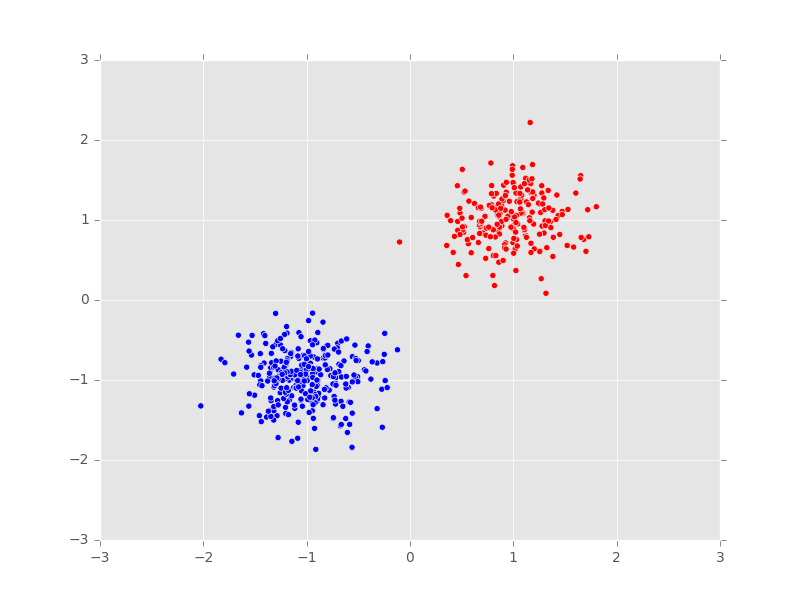
\includegraphics[width=700px]{/images/unsupervised-fig1.png}
